\prob
{
    Find geometric duals of the graphs obtained from $K_5$ and $K_{3,3}$ by
    deleting a single edge of each.
}
\begin{proof}$\,$\pn
    \begin{figure}[H]
        \begin{center}
        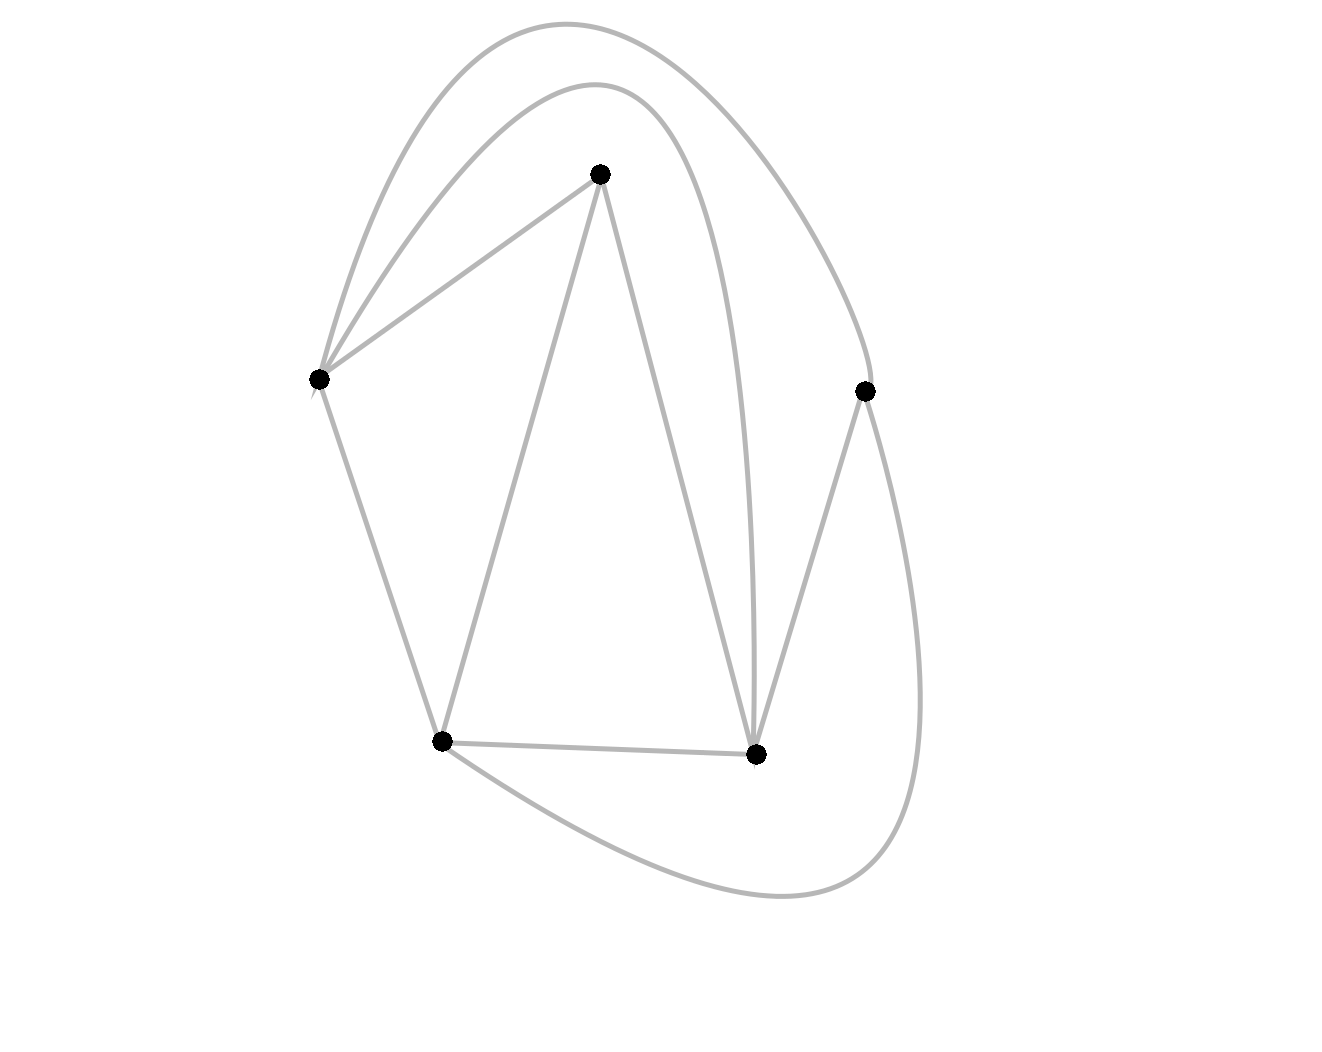
\includegraphics[width=6cm]{Test2/Problem9/PlanarK5WithoutOneEdge.png}
        \end{center}                            
        \caption{$K_5$ without one edge}
        \label{t2:p9_PlanarK5WithoutOneEdge.png}                        
    \end{figure}\pn   
    
    \begin{figure}[H]
        \begin{center}
        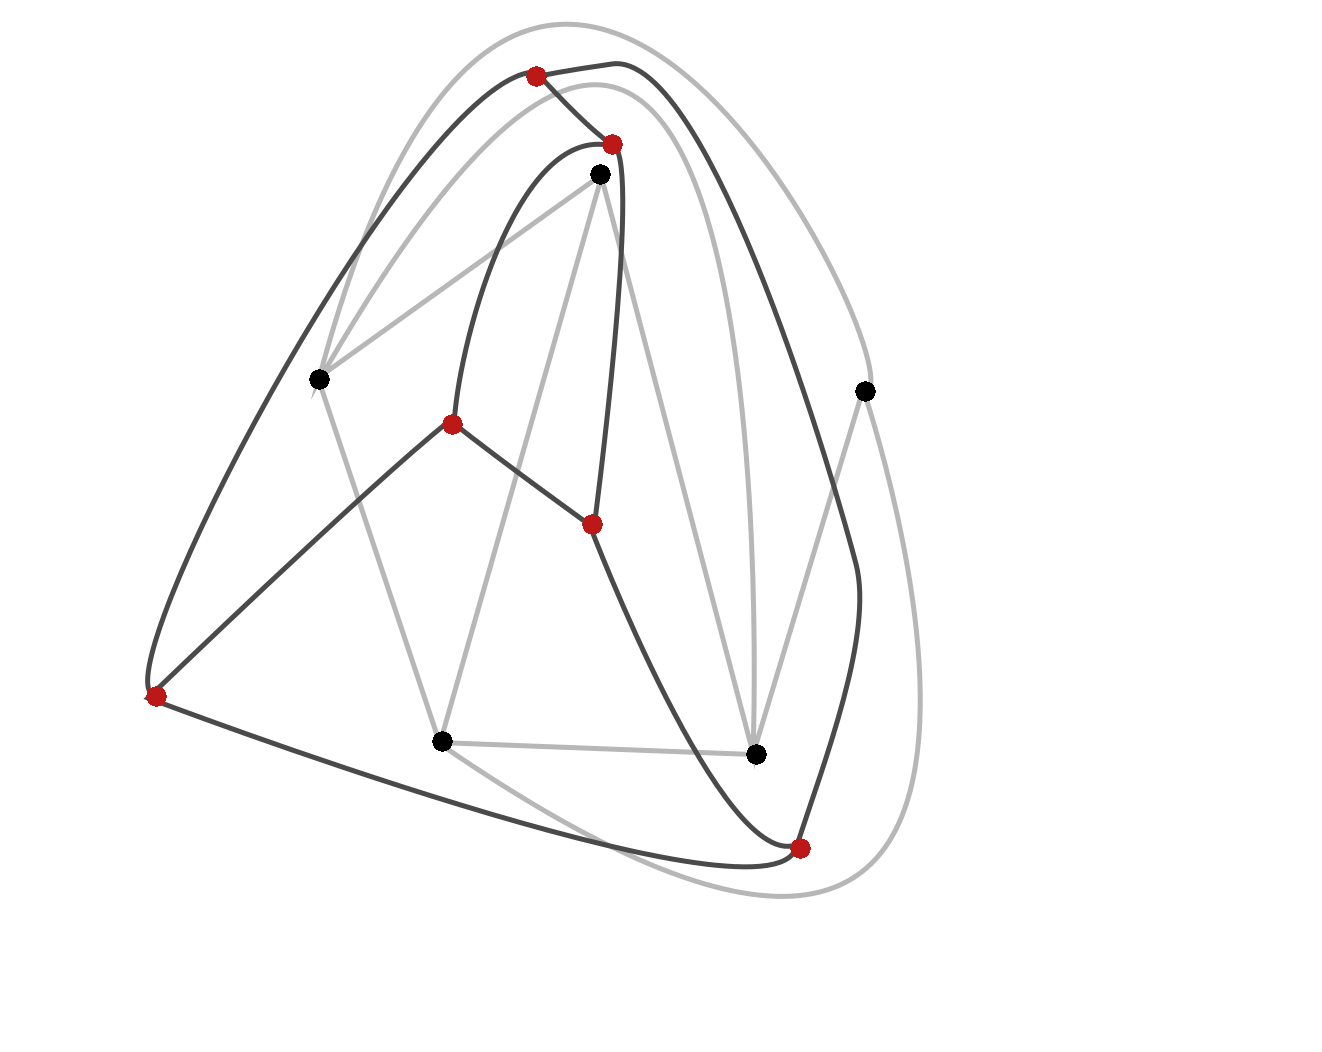
\includegraphics[width=6cm]{Test2/Problem9/PlanarK5WithoutOneEdge_and_dual.png}
        \end{center}                            
        \caption{$K_5$ without one edge and its dual}
        \label{t2:p9_PlanarK5WithoutOneEdge_and_dual.png}                        
    \end{figure}\pn   
    
    \begin{figure}[H]
        \begin{center}
        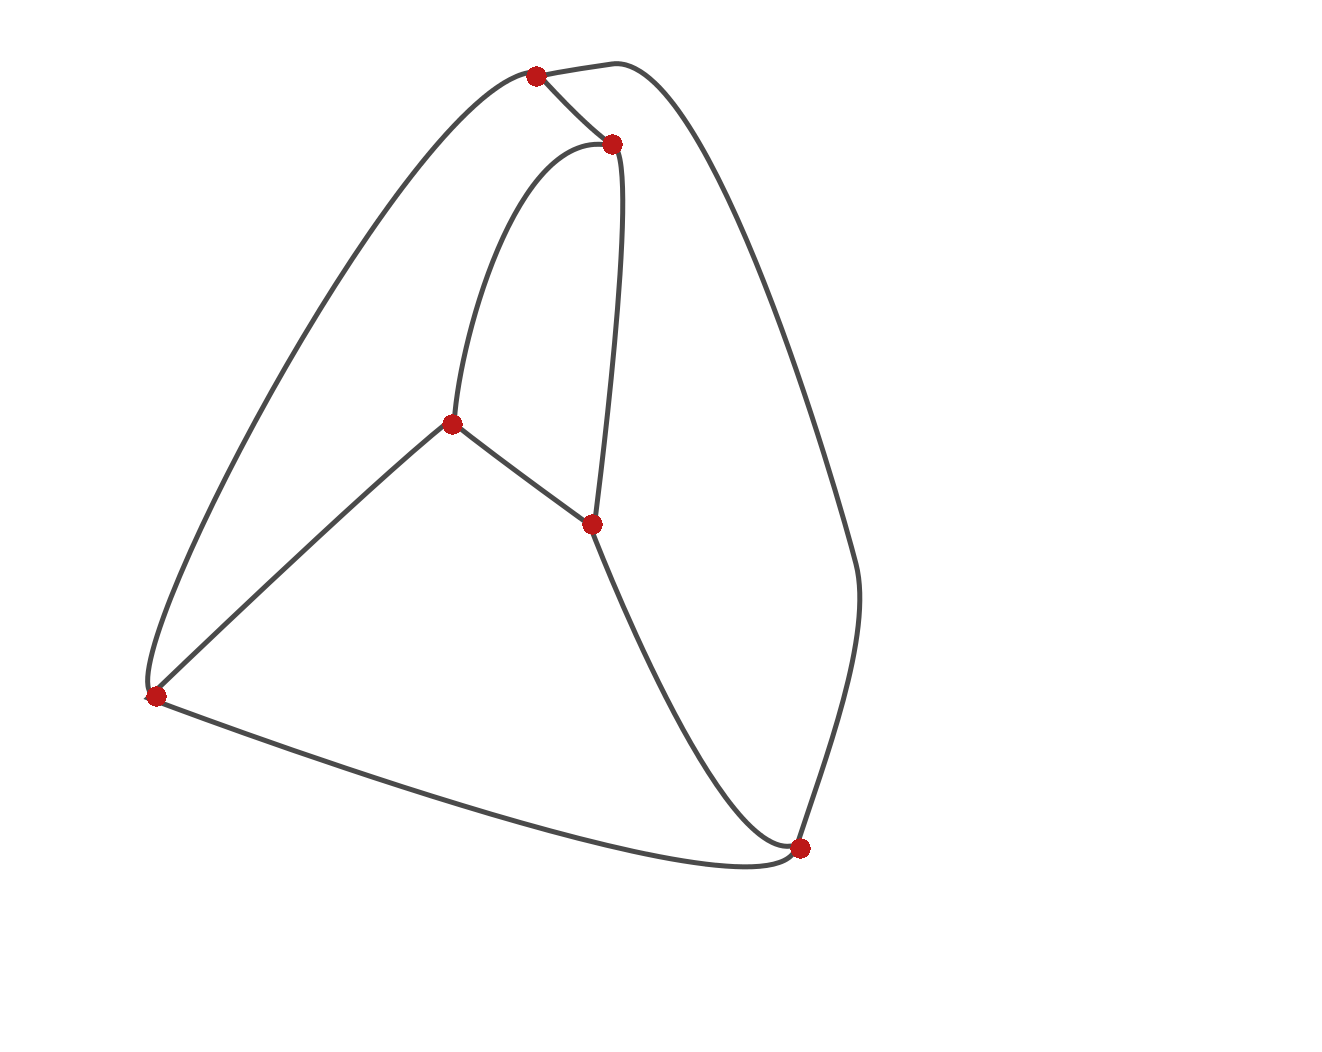
\includegraphics[width=6cm]{Test2/Problem9/PlanarK5WithoutOneEdge_Dual.png}
        \end{center}                            
        \caption{Dual of $K_5$ without one edge}
        \label{t2:p9_PlanarK5WithoutOneEdge_Dual.png}                        
    \end{figure}\pn    
    
    \begin{figure}[H]
        \begin{center}
        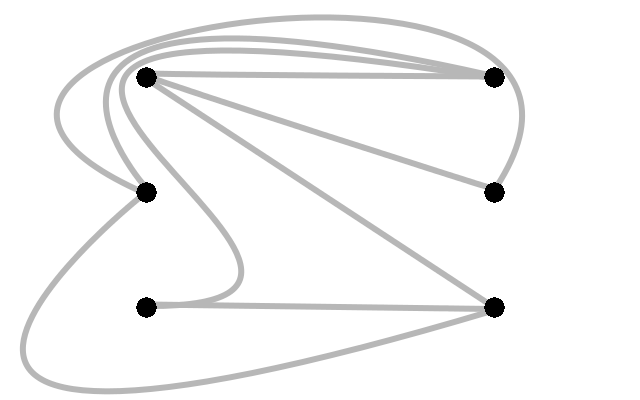
\includegraphics[width=7cm]{Test2/Problem9/PlanarK3_3WithoutOneEdge.png}
        \end{center}                            
        \caption{$K_{3,3}$ without one edge}
        \label{t2:p9_PlanarK3_3WithoutOneEdge.png}                        
    \end{figure}\pn    
    
    \begin{figure}[H]
        \begin{center}
        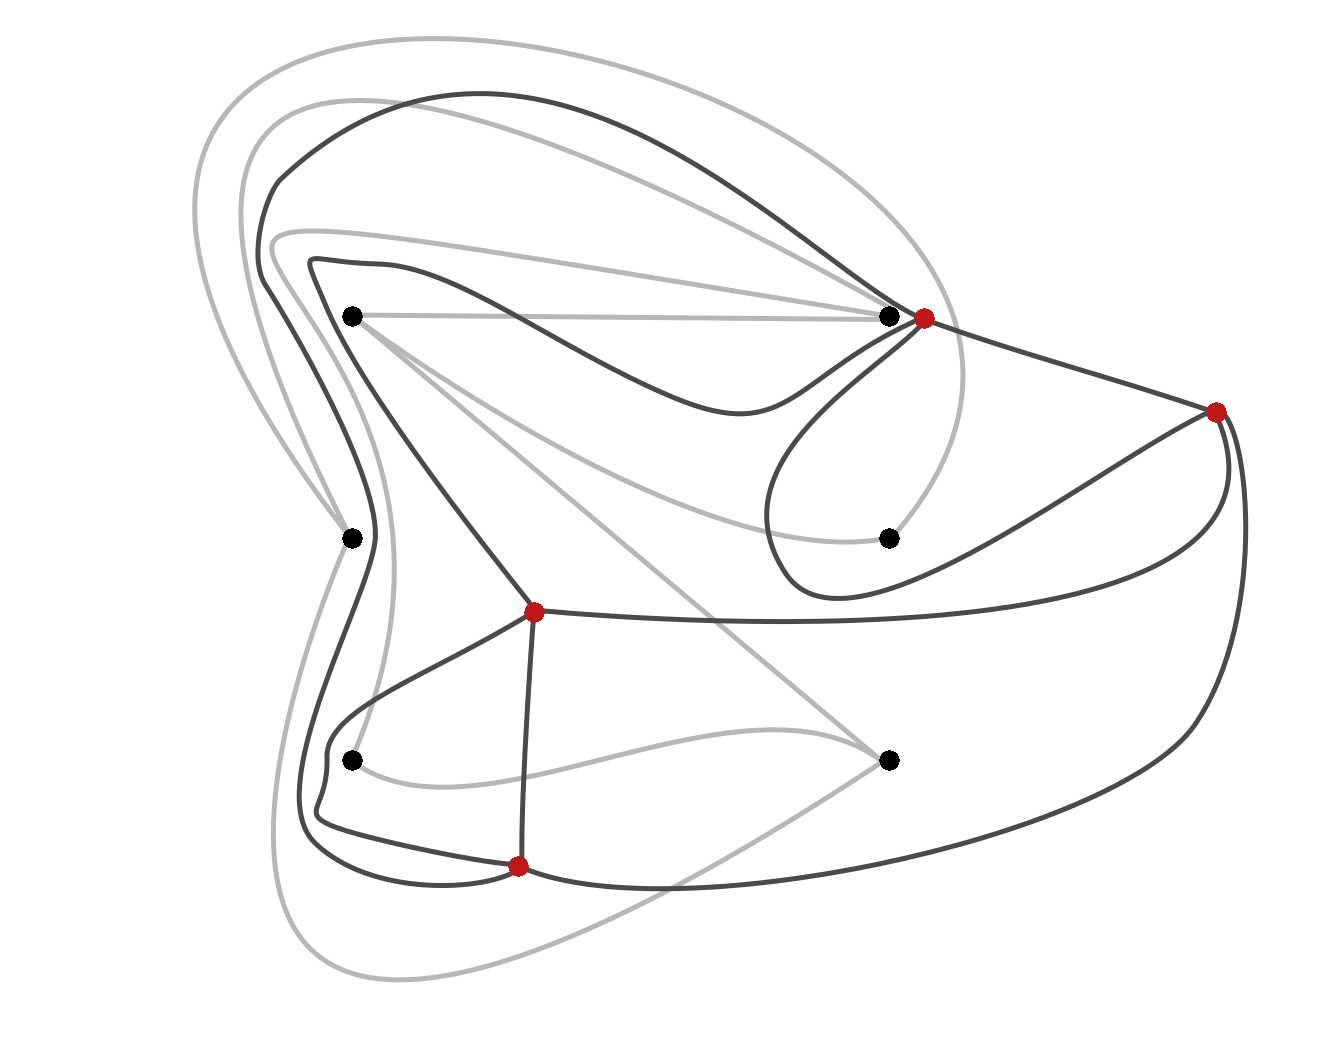
\includegraphics[width=7cm]{Test2/Problem9/PlanarK3_3WithoutOneEdge_and_dual.png}
        \end{center}                            
        \caption{$K_{3,3}$ without one edge and its dual}
        \label{t2:p9_PlanarK3_3WithoutOneEdge_and_dual.png}                        
    \end{figure}\pn    
    
    \begin{figure}[H]
        \begin{center}
        \includegraphics[width=7cm]{Test2/Problem9/PlanarK3_3WithoutOneEdge_dual.png}
        \end{center}                            
        \caption{Dual of $K_{3,3}$ without one edge ($K_4$)}
        \label{t2:p9_PlanarK3_3WithoutOneEdge_dual.png}                        
    \end{figure}\pn
\end{proof}